\apendice{Documentación de usuario}

\section{Introducción}

En este apéndice se explican los conocimientos y requisitos que debe saber el usuario para la utilización del proyecto.

En este apartado no se mencionará el proyecto realizado en Python, puesto que no está orientado al uso por un usuario que no sea desarrollador.
\section{Requisitos de usuarios}
Para que un usuario pueda utilizar la aplicación Android, es necesario:

\begin{itemize}
    \item El usuario disponga con un dispositivo móvil Android con una versión Android 5.0 (Lollipop - API 21) o superior.
    \item El dispositivo debe tener cámara.
    \item El usuario cuente con el hardware externo para obtener fotos de la retina.
    \item La aplicación necesita el permiso para acceder a la cámara y al almacenamiento externo.
    
\end{itemize}

\section{Instalación}
Actualmente solo se dispone de instalación por apk. Para esta instalación, se debe seguir el siguiente procedimiento:
\begin{enumerate}
    \def\labelenumi{\arabic{enumi}.}
    \tightlist
    \item Se debe permitir la instalación de ``origen desconocido''.
    \item Se descarga la apk del repositorio desde el siguiente enlace:
        \url{https://github.com/mfg1014/Retinopatia-diabetica/releases}.
    \item Una vez descargado, se ejecuta el fichero instalable.
    \item Cuando termine su instalación ya se podrá hacer uso de la aplicación.
    
\end{enumerate}
\section{Manual del usuario}

En este apartado, se busca explicar el uso que debería dar el usuario a la aplicación.

\textbf{Navegación por la aplicación}

Al abrir la aplicación, el usuario podrá observar la interfaz de iniciar sesión, donde podrá hacer las siguientes actividades:
\begin{itemize}
    \item Iniciar sesión como invitado, al pulsar esta opción el usuario omite el inicio de sesión y la elección del paciente. Esta opción es la mejor para hacer pruebas o cuando no se poseen los datos del paciente o no se desea almacenar el informe en el paciente.

    \item Iniciar sesión, para ello, el usuario necesita introducir los datos del email y la contraseña; y que estos se encuentren en la base de datos. En caso de que no estén, se mostrará un mensaje de error.

\end{itemize}

Además, el usuario invitado no podrá seleccionar un paciente en específico, y tendrá deshabilitadas todas las opciones de ver datos del paciente y del médico.

Entonces en el diagrama de navegación, visto anteriormente, \ref{fig:diagrama de navegación}, la diferencia se encontraría al iniciar sesión, y luego que el usuario invitado no tendría acceso a la interfaz Datos ni a Perfil.


\textbf{Interfaz seleccionar paciente}

En este caso, se va a considerar que el médico ha iniciado sesión con su email y contraseña, supongamos que estos son medico1\@gmail.com y contrasena, respectivamente.

Entonces al iniciar sesión se le muestra la interfaz para seleccionar paciente; en esta interfaz el usuario deberá seguir este procedimiento:

\begin{enumerate}
    \def\labelenumi{\arabic{enumi}.}
    \tightlist
    \item Introducir un DNI, con solo los números, ejemplo 12345678.
    \item Pulsar el botón ``Lupa'' el cual comprueba si el DNI existe en la base de datos.
    \item Si es el caso, se habilita el botón para entrar al menú principal.
    \item Si se ha introducido un DNI incorrecto, volver a hacer los pasos anteriores.
    \item Pulsar el botón ``Entrar''.
    
\end{enumerate}
\begin{figure}[!ht]
         \centering
         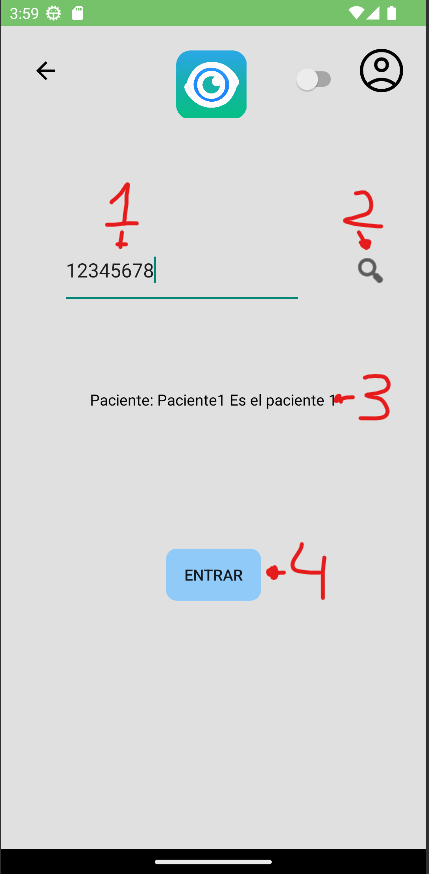
\includegraphics[width=0.45\textwidth]{img/Interfaz seleccionar Paciente.png}
         \caption{Interfaz para seleccionar paciente.}
         \label{fig:InterfazSeleccionarPaciente}
\end{figure}

\textbf{Interfaz foto}

Esta interfaz ya es común para ambos usuarios, su correcto funcionamiento sería:
\begin{enumerate}
    \def\labelenumi{\arabic{enumi}.}
    \tightlist
    \item El usuario escoge entre sacar una foto y elegirla desde la galería.
    \item Una vez hecha la foto, se mostrará en pantalla, y al cabo de unos instantes, habilitará el botón para seleccionar la red neuronal.
    \item Se recomienda al usuario sacar fotos hasta que se consideré de buena calidad, aunque si el médico lo considera buena, pulsar el botón para avanzar a la siguiente interfaz.
\end{enumerate}
\begin{figure}[!ht]
         \centering
         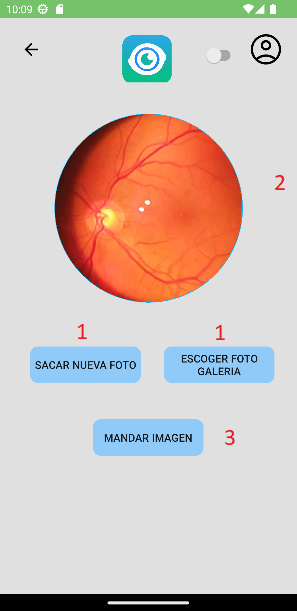
\includegraphics[width=0.45\textwidth]{img/Interfaz FotoApta.png}
         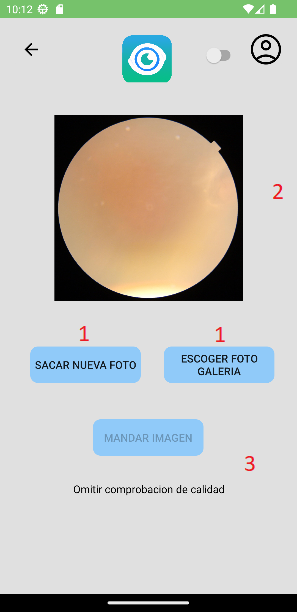
\includegraphics[width=0.45\textwidth]{img/Interfaz FotoNoapta.png}
         \caption{Interfaces para obtener la foto.}
         \label{fig:InterfazFoto}
\end{figure}
\textbf{Interfaz seleccionar red neuronal}

En este caso, esta interfaz no está orientada para el entendimiento del médico puesto que no tiene conocimientos sobre las redes neuronales, pero el objetivo es facilitar estas redes de forma que a lo mejor en una marca de dispositivos una red neuronal obtiene mejor resultados y por tanto, avisar al usuario de cual se recomienda en cada caso:
\begin{enumerate}
    \def\labelenumi{\arabic{enumi}.}
    \tightlist
    \item El usuario escoge las redes neuronales con las que quiera analizar la foto realizada anteriormente
    \item El usuario pulsa el botón ``obtener resultados''.
\end{enumerate}
\begin{figure}[!ht]
         \centering
         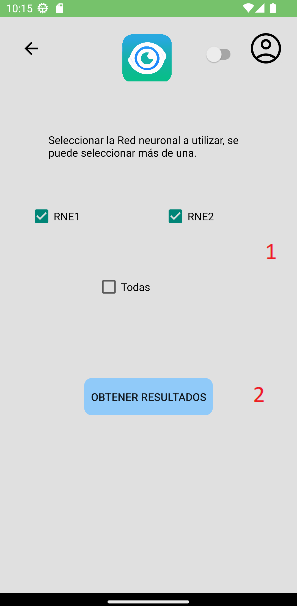
\includegraphics[width=0.45\textwidth]{img/Interfaz seleccionarRNE.png}
         \caption{Interfaz para seleccionar la red.}
         \label{fig:InterfazSeleccionarRNE}
\end{figure}
